\chapter[Contextualização]{Contextualização}

A tramitação de processos no Sistema Judicial brasileiro tem uma característica conhecida nacionalmente por ser bastante lenta, como mostra os dados do \citeonline{cnj-em-numeros}. A evolução da tecnologia e criação da Lei nº \href{planalto.gov.br/ccivil_03/_ato2004-2006/2006/lei/l11419.htm}{11.419} permitiu que se alterasse o paradigma de trabalho que os juristas e seus auxiliares estavam acostumados, com a informatização de processos para um meio eletrônico.

Porém, a mudança desse modelo de trabalho não foi instantânea e muitos processos físicos já existentes ainda não haviam sido extintos\footnote{
    O Código do Processo Civil (CPC) caracteriza um processo extinto como um processo cujo sua ação já foi finalizada, ou seja, chegou ao seu fim.
} e ainda estavam em tramitação. Com isso, os tribunais de todo o país começaram uma força-tarefa para realizar a digitalização dos processos e aloca-los para um sistema informatizado, criando-se então o Processo Judicial Eletrônico como sendo a plataforma que visa possibilitar a "completa substituição do meio físico papel pelos meios de armazenamento disponibilizados pela informática" \cite{pje-e-sua-implantacao}. Porém, por se tratar de um enorme volume processual, a quantidade de páginas para serem escaneadas chegam a números assustadores e a possibilidade de haverem erros no processo de digitalização aumenta com o trabalho excessivo e manual, diminuindo consequentemente a qualidade dos textos digitalizados.

\begin{figure}[H]
    \centering
    \caption{Exemplo de escaneamento de documento com erros humanos/de máquina.}
    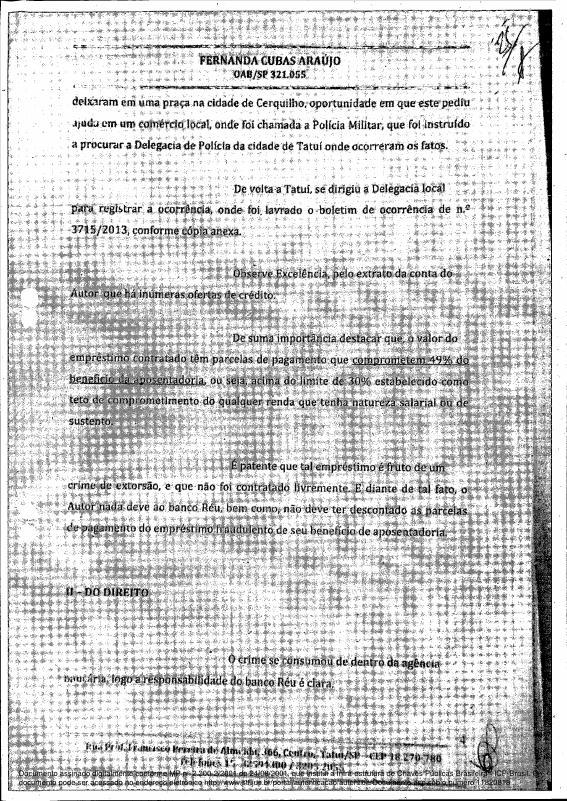
\includegraphics[scale=0.3]{figuras/badly-scanned-image.jpg}
    \legend{Fonte: STF.}
    \label{fig:badly-scanned-image}
\end{figure}

\section{Problemática}

Com os processos jurídicos em uma plataforma informatizada e o crescimento na área de \textit{Machine Learning} voltada para o processamento de imagens e processamento de texto com Processamento de Linguagem Natural, muitas empresas viram uma grande oportunidade no mercado: aplicar Inteligência Artificial na área jurídica. Com isso, empresas e projetos de pesquisa começaram a surgir como por exemplo o Projeto Victor \cite{cnn-for-STF} desenvolvido pelos integrantes do grupo GPAM da Universidade de Brasília. O projeto consistiu em criar um modelo para classificação das repercussões gerais do Supremo Tribunal Federal.

Em sua etapa de desenvolvimento, era necessário extrair informaçõs dos documentos presentes nos diversos processos, sendo esses podendo ser imagens escaneadas ou digitalizadas, sendo necessário aplicar tecnologias de extração de texto a partir de imagem, \textit{Optical Character Recognition}, o que foi identificado como problemático no decorrer do projeto \cite{cnn-for-STF}.

Existem diversos tipos de filtros de imagens que podem ser aplicados para auxiliar os algoritmos de OCR a atingirem melhores resultados. Um exemplo é a binarização, a qual coloca todos os pixels da imagem para valores de 255 (preto) ou 0 (branco), para melhor distinguir as letras dos valores esparços em branco da imagem \cite{image-binarization}, dando mais destaque entre pixels pretos e brancos. Porém, dependendo do valor do pixel encontrado na imagem manchada, como a figura \ref{fig:badly-scanned-image} isso pode não ser solucionado, tendo que optar por outros filtros como alternativa.

\begin{figure}[H]
    \centering
    \caption{Aplicação de filtro de binarização na figura \ref{fig:badly-scanned-image}.}
    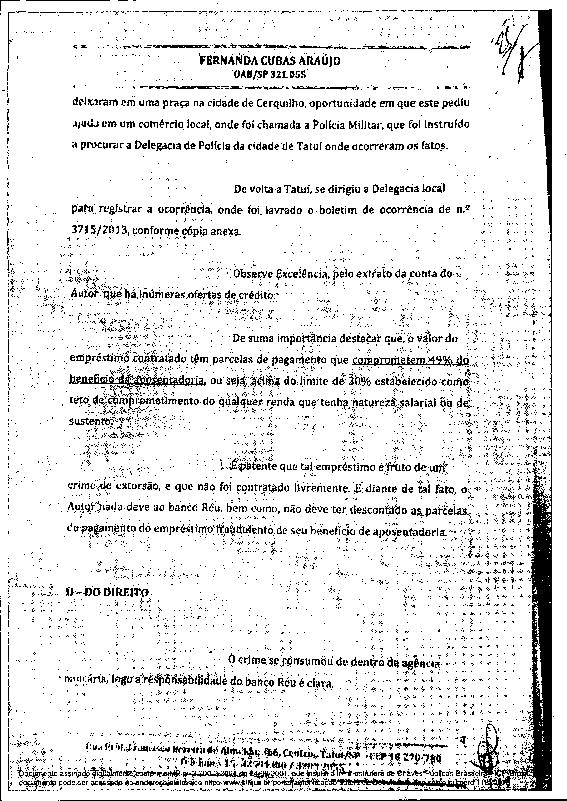
\includegraphics[scale=0.3]{figuras/binarized-badly-scanned-image.jpg}
    \legend{Fonte: Autoral.}
    \label{fig:binarized-badly-scanned-image}
\end{figure}

Com uma aproximação na imagem, é possível verificar que, mesmo com o filtro de binarização, parte da imagem não fica visível, impedindo assim a extração de informação dessa imagem da maneira a qual ela se encontra.

\begin{figure}[H]
    \centering
    \caption{Aproximação em parte da imagem binarizada apresentada na figura \ref{fig:binarized-badly-scanned-image}.}
    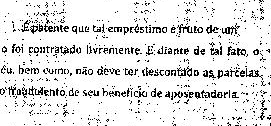
\includegraphics[scale=1]{figuras/zoom-in-binarized-image.png}
    \legend{Fonte: Autoral.}
    \label{fig:zoom-in-binarized-image}
\end{figure}

Idealiza-se então criar um modelo de ML que consiga, a partir de uma imagem ruim como foi apresentada na figura \ref{fig:badly-scanned-image} seja possível corrigir os erros apresentados nessa imagem que permita os algoritmos de extração de texto de imagem atingirem melhores resultados.